\documentclass[tikz,border=12pt]{standalone}
\usepackage{xcolor}
\usepackage{amsmath,amssymb}
\usepackage{microtype}
\usetikzlibrary{shapes,arrows.meta,positioning,calc,fit,backgrounds}

% ─── Color Palette (High Visibility & Standardized Academic) ────────────────
\definecolor{headerNavy}{RGB}{15, 23, 42}
\definecolor{busSlate}{RGB}{71, 85, 105}
\definecolor{textDark}{RGB}{15, 23, 42}
\definecolor{textSub}{RGB}{71, 85, 105}

% Stage 1: Acquisition (Teal)
\definecolor{cTealBorder}{RGB}{13, 148, 136}
\definecolor{cTealBg}{RGB}{240, 253, 250}
\definecolor{cTealBadge}{RGB}{15, 118, 110}

% Stage 2: Preprocessing (Slate)
\definecolor{cSlateBorder}{RGB}{71, 85, 105}
\definecolor{cSlateBg}{RGB}{248, 250, 252}
\definecolor{cSlateBadge}{RGB}{51, 65, 85}

% Stage 3: Extraction (Cobalt)
\definecolor{cBlueBorder}{RGB}{37, 99, 235}
\definecolor{cBlueBg}{RGB}{239, 246, 255}
\definecolor{cBlueBadge}{RGB}{29, 78, 216}

% Stage 4: Projection (Amber)
\definecolor{cAmberBorder}{RGB}{217, 119, 6}
\definecolor{cAmberBg}{RGB}{255, 251, 235}
\definecolor{cAmberBadge}{RGB}{180, 83, 9}

% Stage 5: Clustering (Emerald)
\definecolor{cGreenBorder}{RGB}{16, 185, 129}
\definecolor{cGreenBg}{RGB}{236, 253, 245}
\definecolor{cGreenBadge}{RGB}{5, 150, 105}

% Stage 6: Interpretation (Purple)
\definecolor{cPurpleBorder}{RGB}{139, 92, 246}
\definecolor{cPurpleBg}{RGB}{245, 243, 255}
\definecolor{cPurpleBadge}{RGB}{109, 40, 217}

% Stage 7: Validation (Rose)
\definecolor{cRoseBorder}{RGB}{225, 29, 72}
\definecolor{cRoseBg}{RGB}{255, 241, 242}
\definecolor{cRoseBadge}{RGB}{190, 18, 60}

\begin{document}
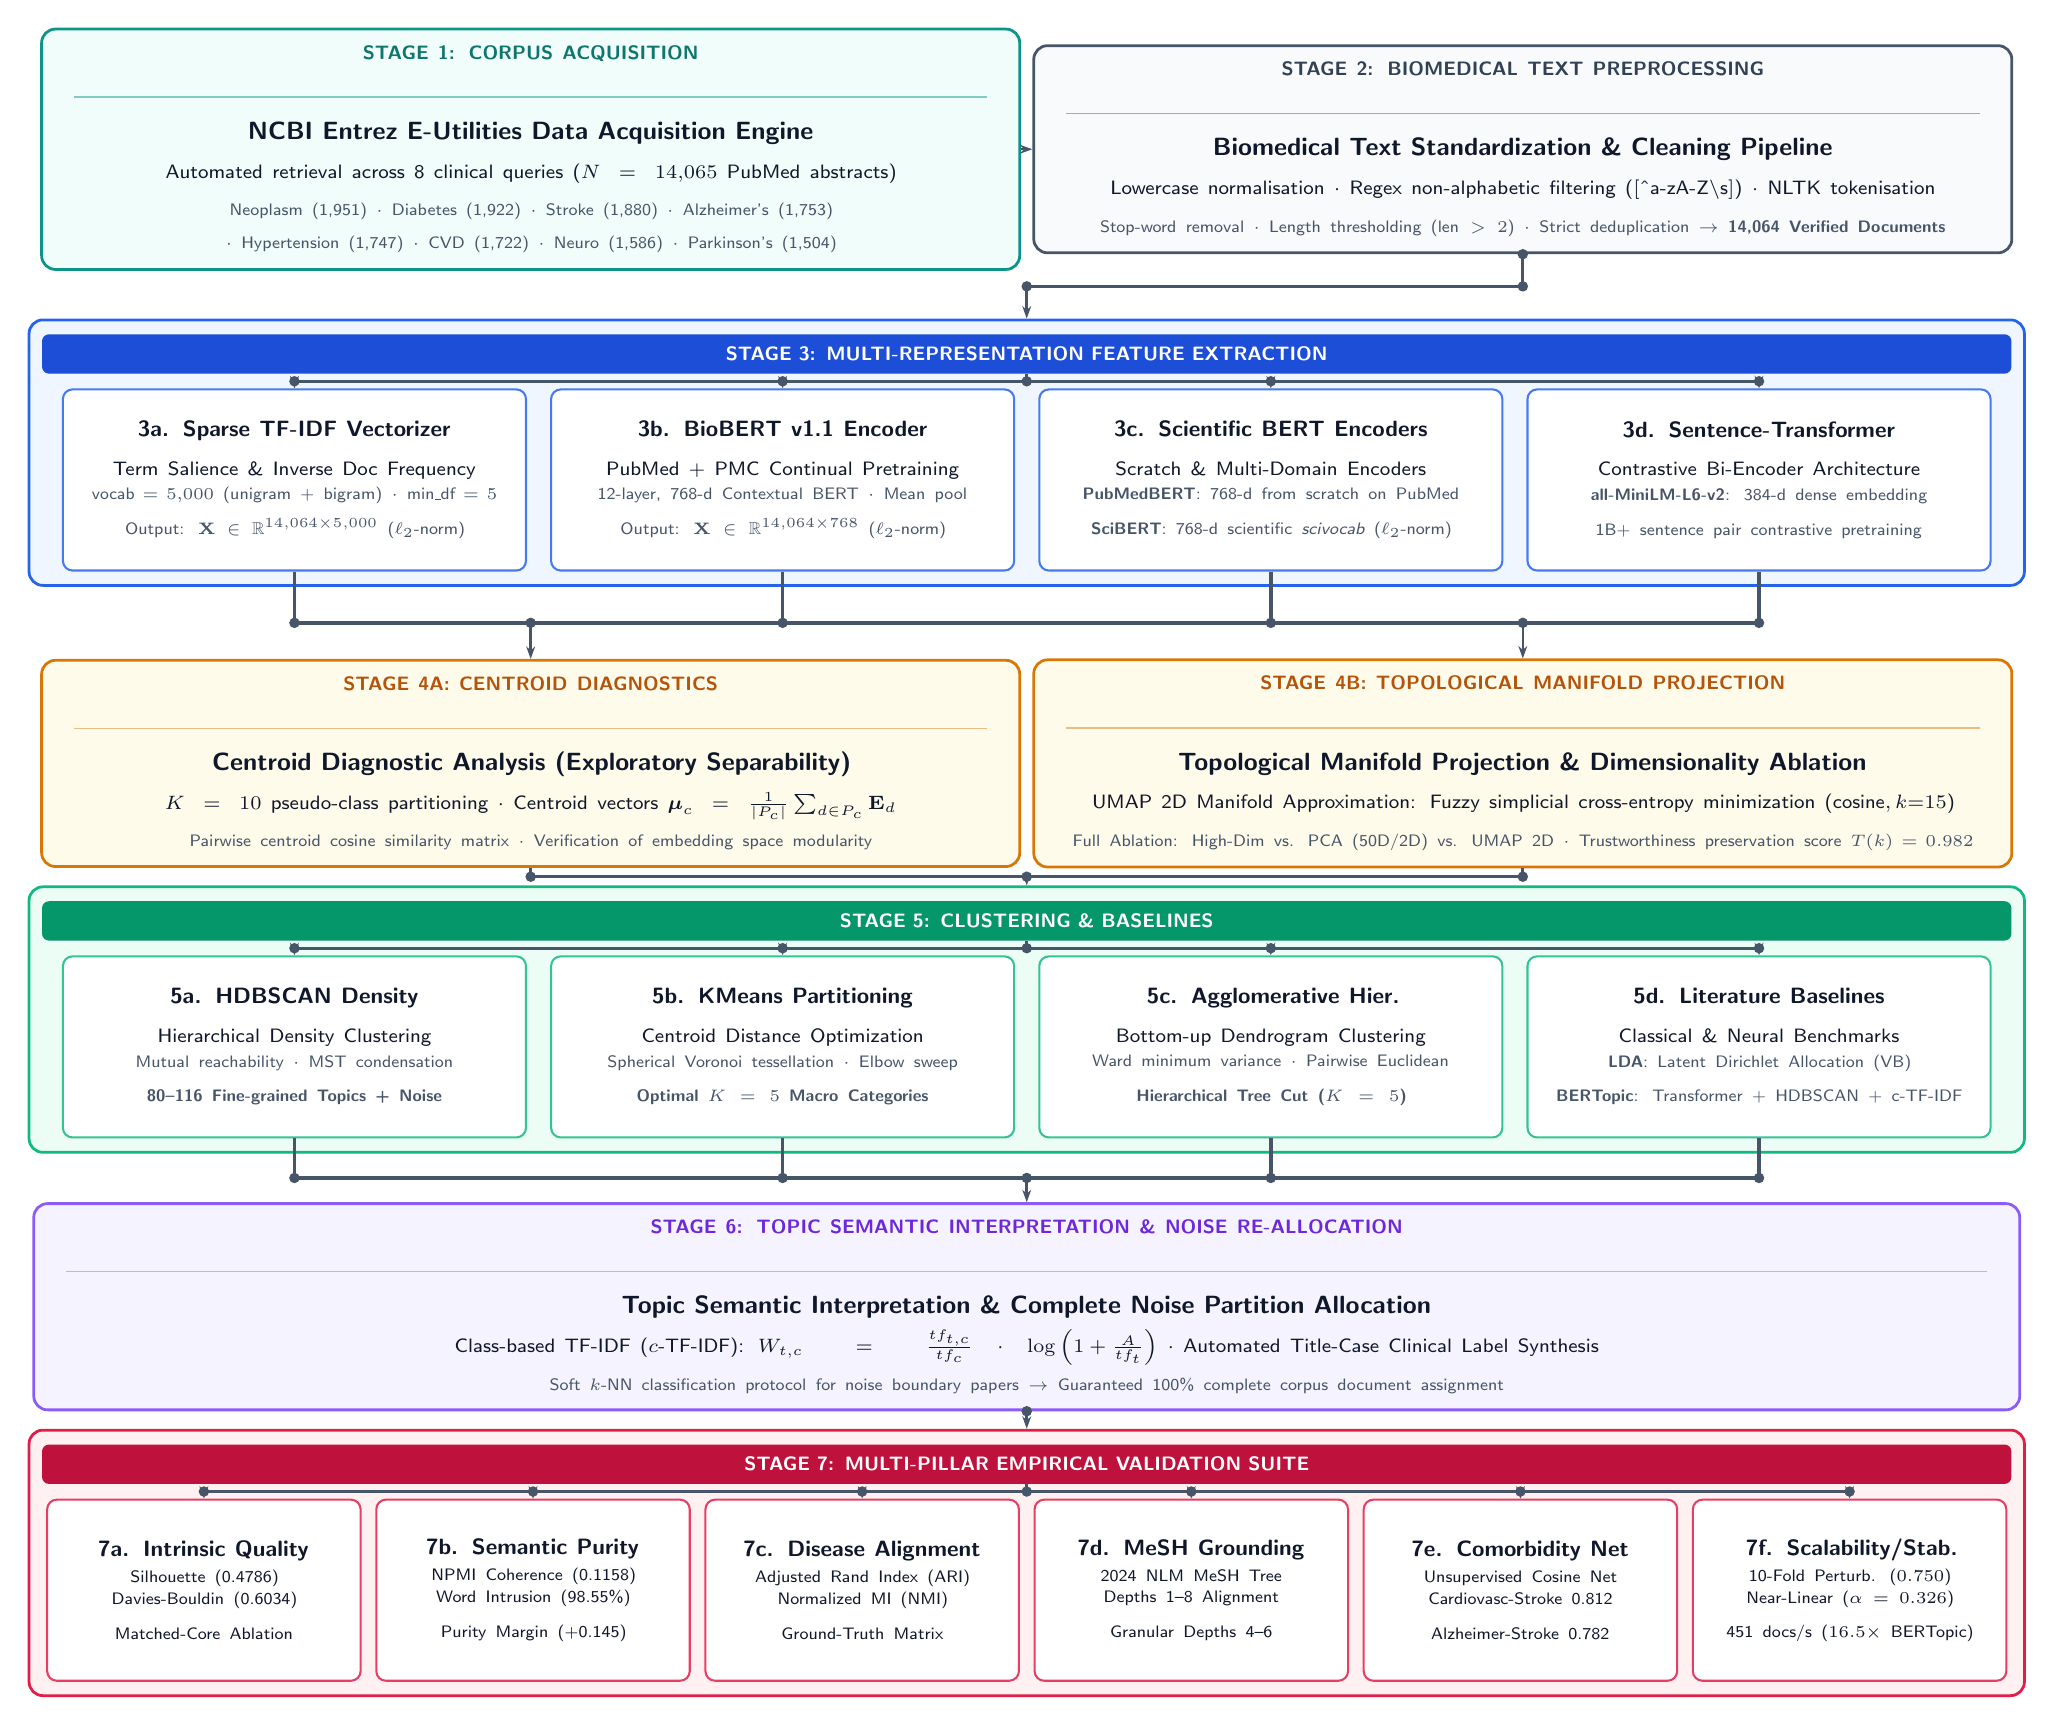
\begin{tikzpicture}[
  font=\sffamily,
  >=Stealth,
  card/.style={draw=#1Border, fill=#1Bg, line width=1.0pt, rounded corners=5pt, align=center, inner sep=6pt, text=textDark},
  subcard/.style={draw=#1Border!85, fill=white, line width=0.75pt, rounded corners=3.5pt, align=center, inner sep=4pt, text=textDark},
  headerBar/.style={fill=#1Badge, text=white, font=\sffamily\bfseries\fontsize{7pt}{8.5pt}\selectfont, rounded corners=2.5pt, inner sep=3pt, minimum height=5mm, align=center},
  bus/.style={line width=1.2pt, draw=busSlate},
  branch/.style={-{Stealth[length=4.5pt, width=3.2pt]}, line width=0.9pt, draw=busSlate},
  junc/.style={circle, fill=busSlate, inner sep=0pt, minimum size=3.8pt}
]

\coordinate (originX) at (0,0);

% ─── ROW 1: ACQUISITION & PREPROCESSING ─────────────────────────────────────
\node[card=cTeal, text width=120mm, minimum height=24mm] (cStage1) at (-63mm, 0) {
  {\color{cTealBadge}\bfseries\fontsize{7.5pt}{9pt}\selectfont STAGE 1: CORPUS ACQUISITION}\\[2pt]
  {\color{cTealBorder!50}\rule{116mm}{0.5pt}}\\[3pt]
  {\fontsize{8.8pt}{10.5pt}\selectfont\textbf{NCBI Entrez E-Utilities Data Acquisition Engine}}\\[2pt]
  {\fontsize{7.2pt}{8.6pt}\selectfont Automated retrieval across 8 clinical queries ($N = 14{,}065$ PubMed abstracts)}\\[1.5pt]
  {\fontsize{6.3pt}{7.5pt}\selectfont\color{textSub} Neoplasm (1,951) $\cdot$ Diabetes (1,922) $\cdot$ Stroke (1,880) $\cdot$ Alzheimer's (1,753) $\cdot$ Hypertension (1,747) $\cdot$ CVD (1,722) $\cdot$ Neuro (1,586) $\cdot$ Parkinson's (1,504)}
};

\node[card=cSlate, text width=120mm, minimum height=24mm] (cStage2) at (63mm, 0) {
  {\color{cSlateBadge}\bfseries\fontsize{7.5pt}{9pt}\selectfont STAGE 2: BIOMEDICAL TEXT PREPROCESSING}\\[2pt]
  {\color{cSlateBorder!50}\rule{116mm}{0.5pt}}\\[3pt]
  {\fontsize{8.8pt}{10.5pt}\selectfont\textbf{Biomedical Text Standardization \& Cleaning Pipeline}}\\[2pt]
  {\fontsize{7.2pt}{8.6pt}\selectfont Lowercase normalisation $\cdot$ Regex non-alphabetic filtering ($[\text{\textasciicircum a-zA-Z}\backslash\text{s}]$) $\cdot$ NLTK tokenisation}\\[1.5pt]
  {\fontsize{6.3pt}{7.5pt}\selectfont\color{textSub} Stop-word removal $\cdot$ Length thresholding ($\text{len} > 2$) $\cdot$ Strict deduplication $\rightarrow$ \textbf{14{,}064 Verified Documents}}
};

\draw[branch] (cStage1.east) -- (cStage2.west);

% ─── ROW 2: MULTI-REPRESENTATION EXTRACTION ─────────────────────────────────
\coordinate (r2Center) at (0, -42mm);

% Internal Header Bar for Stage 3
\node[headerBar=cBlue, text width=248mm] (hStage3) at ($(r2Center) + (0, 16mm)$) {STAGE 3: MULTI-REPRESENTATION FEATURE EXTRACTION};

\node[subcard=cBlue, text width=56mm, minimum height=23mm] at ($(r2Center) + (-93mm, 0)$) (c3a) {
  {\fontsize{8.2pt}{9.8pt}\selectfont\textbf{3a. Sparse TF-IDF Vectorizer}}\\[2pt]
  {\fontsize{6.8pt}{8.2pt}\selectfont Term Salience \& Inverse Doc Frequency}\\[1.5pt]
  {\fontsize{6.2pt}{7.4pt}\selectfont\color{textSub} $\text{vocab} = 5{,}000$ (unigram + bigram) $\cdot$ $\text{min\_df} = 5$\\[0.5pt] Output: $\mathbf{X} \in \mathbb{R}^{14{,}064 \times 5{,}000}$ ($\ell_2$-norm)}
};

\node[subcard=cBlue, text width=56mm, minimum height=23mm] at ($(r2Center) + (-31mm, 0)$) (c3b) {
  {\fontsize{8.2pt}{9.8pt}\selectfont\textbf{3b. BioBERT v1.1 Encoder}}\\[2pt]
  {\fontsize{6.8pt}{8.2pt}\selectfont PubMed + PMC Continual Pretraining}\\[1.5pt]
  {\fontsize{6.2pt}{7.4pt}\selectfont\color{textSub} 12-layer, 768-d Contextual BERT $\cdot$ Mean pool\\[0.5pt] Output: $\mathbf{X} \in \mathbb{R}^{14{,}064 \times 768}$ ($\ell_2$-norm)}
};

\node[subcard=cBlue, text width=56mm, minimum height=23mm] at ($(r2Center) + (31mm, 0)$) (c3c) {
  {\fontsize{8.2pt}{9.8pt}\selectfont\textbf{3c. Scientific BERT Encoders}}\\[2pt]
  {\fontsize{6.8pt}{8.2pt}\selectfont Scratch \& Multi-Domain Encoders}\\[1.5pt]
  {\fontsize{6.2pt}{7.4pt}\selectfont\color{textSub} \textbf{PubMedBERT}: 768-d from scratch on PubMed\\[0.5pt] \textbf{SciBERT}: 768-d scientific \textit{scivocab} ($\ell_2$-norm)}
};

\node[subcard=cBlue, text width=56mm, minimum height=23mm] at ($(r2Center) + (93mm, 0)$) (c3d) {
  {\fontsize{8.2pt}{9.8pt}\selectfont\textbf{3d. Sentence-Transformer}}\\[2pt]
  {\fontsize{6.8pt}{8.2pt}\selectfont Contrastive Bi-Encoder Architecture}\\[1.5pt]
  {\fontsize{6.2pt}{7.4pt}\selectfont\color{textSub} \textbf{all-MiniLM-L6-v2}: 384-d dense embedding\\[0.5pt] 1B+ sentence pair contrastive pretraining}
};

\begin{scope}[on background layer]
  \node[card=cBlue, inner xsep=4.5pt, inner ysep=5pt, fit=(hStage3) (c3a) (c3d)] (boxStage3) {};
\end{scope}

% ─── ROW 3: DIAGNOSTIC & TOPOLOGICAL REDUCTION ──────────────────────────────
\coordinate (r3Center) at (0, -78mm);

\node[card=cAmber, text width=120mm, minimum height=24mm] at ($(r3Center) + (-63mm, 0)$) (c4a) {
  {\color{cAmberBadge}\bfseries\fontsize{7.5pt}{9pt}\selectfont STAGE 4A: CENTROID DIAGNOSTICS}\\[2pt]
  {\color{cAmberBorder!50}\rule{116mm}{0.5pt}}\\[3pt]
  {\fontsize{8.8pt}{10.5pt}\selectfont\textbf{Centroid Diagnostic Analysis (Exploratory Separability)}}\\[2pt]
  {\fontsize{7.2pt}{8.6pt}\selectfont $K = 10$ pseudo-class partitioning $\cdot$ Centroid vectors $\boldsymbol{\mu}_c = \frac{1}{|P_c|}\sum_{d \in P_c}\mathbf{E}_d$}\\[1.5pt]
  {\fontsize{6.3pt}{7.5pt}\selectfont\color{textSub} Pairwise centroid cosine similarity matrix $\cdot$ Verification of embedding space modularity}
};

\node[card=cAmber, text width=120mm, minimum height=24mm] at ($(r3Center) + (63mm, 0)$) (c4b) {
  {\color{cAmberBadge}\bfseries\fontsize{7.5pt}{9pt}\selectfont STAGE 4B: TOPOLOGICAL MANIFOLD PROJECTION}\\[2pt]
  {\color{cAmberBorder!50}\rule{116mm}{0.5pt}}\\[3pt]
  {\fontsize{8.8pt}{10.5pt}\selectfont\textbf{Topological Manifold Projection \& Dimensionality Ablation}}\\[2pt]
  {\fontsize{7.2pt}{8.6pt}\selectfont UMAP 2D Manifold Approximation: Fuzzy simplicial cross-entropy minimization ($\text{cosine}, k{=}15$)}\\[1.5pt]
  {\fontsize{6.3pt}{7.5pt}\selectfont\color{textSub} Full Ablation: High-Dim vs. PCA (50D/2D) vs. UMAP 2D $\cdot$ Trustworthiness preservation score $T(k) = 0.982$}
};

% ─── ROW 4: CLUSTERING & BASELINES ──────────────────────────────────────────
\coordinate (r4Center) at (0, -114mm);

% Internal Header Bar for Stage 5
\node[headerBar=cGreen, text width=248mm] (hStage5) at ($(r4Center) + (0, 16mm)$) {STAGE 5: CLUSTERING \& BASELINES};

\node[subcard=cGreen, text width=56mm, minimum height=23mm] at ($(r4Center) + (-93mm, 0)$) (c5a) {
  {\fontsize{8.2pt}{9.8pt}\selectfont\textbf{5a. HDBSCAN Density}}\\[2pt]
  {\fontsize{6.8pt}{8.2pt}\selectfont Hierarchical Density Clustering}\\[1.5pt]
  {\fontsize{6.2pt}{7.4pt}\selectfont\color{textSub} Mutual reachability $\cdot$ MST condensation\\[0.5pt] \textbf{80--116 Fine-grained Topics + Noise}}
};

\node[subcard=cGreen, text width=56mm, minimum height=23mm] at ($(r4Center) + (-31mm, 0)$) (c5b) {
  {\fontsize{8.2pt}{9.8pt}\selectfont\textbf{5b. KMeans Partitioning}}\\[2pt]
  {\fontsize{6.8pt}{8.2pt}\selectfont Centroid Distance Optimization}\\[1.5pt]
  {\fontsize{6.2pt}{7.4pt}\selectfont\color{textSub} Spherical Voronoi tessellation $\cdot$ Elbow sweep\\[0.5pt] \textbf{Optimal $K = 5$ Macro Categories}}
};

\node[subcard=cGreen, text width=56mm, minimum height=23mm] at ($(r4Center) + (31mm, 0)$) (c5c) {
  {\fontsize{8.2pt}{9.8pt}\selectfont\textbf{5c. Agglomerative Hier.}}\\[2pt]
  {\fontsize{6.8pt}{8.2pt}\selectfont Bottom-up Dendrogram Clustering}\\[1.5pt]
  {\fontsize{6.2pt}{7.4pt}\selectfont\color{textSub} Ward minimum variance $\cdot$ Pairwise Euclidean\\[0.5pt] \textbf{Hierarchical Tree Cut ($K = 5$)}}
};

\node[subcard=cGreen, text width=56mm, minimum height=23mm] at ($(r4Center) + (93mm, 0)$) (c5d) {
  {\fontsize{8.2pt}{9.8pt}\selectfont\textbf{5d. Literature Baselines}}\\[2pt]
  {\fontsize{6.8pt}{8.2pt}\selectfont Classical \& Neural Benchmarks}\\[1.5pt]
  {\fontsize{6.2pt}{7.4pt}\selectfont\color{textSub} \textbf{LDA}: Latent Dirichlet Allocation (VB)\\[0.5pt] \textbf{BERTopic}: Transformer + HDBSCAN + c-TF-IDF}
};

\begin{scope}[on background layer]
  \node[card=cGreen, inner xsep=4.5pt, inner ysep=5pt, fit=(hStage5) (c5a) (c5d)] (boxStage5) {};
\end{scope}

% ─── ROW 5: TOPIC INTERPRETATION ───────────────────────────────────────────
\coordinate (r5Center) at (0, -147mm);

\node[card=cPurple, text width=248mm, minimum height=22mm] at (r5Center) (cStage6) {
  {\color{cPurpleBadge}\bfseries\fontsize{7.5pt}{9pt}\selectfont STAGE 6: TOPIC SEMANTIC INTERPRETATION \& NOISE RE-ALLOCATION}\\[2pt]
  {\color{cPurpleBorder!50}\rule{244mm}{0.5pt}}\\[3pt]
  {\fontsize{8.8pt}{10.5pt}\selectfont\textbf{Topic Semantic Interpretation \& Complete Noise Partition Allocation}}\\[2pt]
  {\fontsize{7.2pt}{8.6pt}\selectfont Class-based TF-IDF ($c\text{-TF-IDF}$): $W_{t,c} = \frac{tf_{t,c}}{tf_c} \cdot \log\left(1 + \frac{A}{tf_t}\right)$ $\cdot$ Automated Title-Case Clinical Label Synthesis}\\[1.5pt]
  {\fontsize{6.3pt}{7.5pt}\selectfont\color{textSub} Soft $k$-NN classification protocol for noise boundary papers $\rightarrow$ Guaranteed 100\% complete corpus document assignment}
};

% ─── ROW 6: MULTI-PILLAR EMPIRICAL VALIDATION SUITE ────────────────────────
\coordinate (r6Center) at (0, -183mm);

% Internal Header Bar for Stage 7
\node[headerBar=cRose, text width=248mm] (hStage7) at ($(r6Center) + (0, 16mm)$) {STAGE 7: MULTI-PILLAR EMPIRICAL VALIDATION SUITE};

\node[subcard=cRose, text width=37mm, minimum height=23mm] at ($(r6Center) + (-104.5mm, 0)$) (c7a) {
  {\fontsize{7.8pt}{9.2pt}\selectfont\textbf{7a. Intrinsic Quality}}\\[2pt]
  {\fontsize{6.2pt}{7.4pt}\selectfont Silhouette (0.4786)\\[0.5pt] Davies-Bouldin (0.6034)\\[0.5pt] Matched-Core Ablation}
};

\node[subcard=cRose, text width=37mm, minimum height=23mm] at ($(r6Center) + (-62.7mm, 0)$) (c7b) {
  {\fontsize{7.8pt}{9.2pt}\selectfont\textbf{7b. Semantic Purity}}\\[2pt]
  {\fontsize{6.2pt}{7.4pt}\selectfont NPMI Coherence (0.1158)\\[0.5pt] Word Intrusion (98.55\%)\\[0.5pt] Purity Margin (+0.145)}
};

\node[subcard=cRose, text width=37mm, minimum height=23mm] at ($(r6Center) + (-20.9mm, 0)$) (c7c) {
  {\fontsize{7.8pt}{9.2pt}\selectfont\textbf{7c. Disease Alignment}}\\[2pt]
  {\fontsize{6.2pt}{7.4pt}\selectfont Adjusted Rand Index (ARI)\\[0.5pt] Normalized MI (NMI)\\[0.5pt] Ground-Truth Matrix}
};

\node[subcard=cRose, text width=37mm, minimum height=23mm] at ($(r6Center) + (20.9mm, 0)$) (c7d) {
  {\fontsize{7.8pt}{9.2pt}\selectfont\textbf{7d. MeSH Grounding}}\\[2pt]
  {\fontsize{6.2pt}{7.4pt}\selectfont 2024 NLM MeSH Tree\\[0.5pt] Depths 1--8 Alignment\\[0.5pt] Granular Depths 4--6}
};

\node[subcard=cRose, text width=37mm, minimum height=23mm] at ($(r6Center) + (62.7mm, 0)$) (c7e) {
  {\fontsize{7.8pt}{9.2pt}\selectfont\textbf{7e. Comorbidity Net}}\\[2pt]
  {\fontsize{6.2pt}{7.4pt}\selectfont Unsupervised Cosine Net\\[0.5pt] Cardiovasc-Stroke 0.812\\[0.5pt] Alzheimer-Stroke 0.782}
};

\node[subcard=cRose, text width=37mm, minimum height=23mm] at ($(r6Center) + (104.5mm, 0)$) (c7f) {
  {\fontsize{7.8pt}{9.2pt}\selectfont\textbf{7f. Scalability/Stab.}}\\[2pt]
  {\fontsize{6.2pt}{7.4pt}\selectfont 10-Fold Perturb. ($0.750$)\\[0.5pt] Near-Linear ($\alpha = 0.326$)\\[0.5pt] 451 docs/s ($16.5\times$ BERTopic)}
};

\begin{scope}[on background layer]
  \node[card=cRose, inner xsep=4.5pt, inner ysep=5pt, fit=(hStage7) (c7a) (c7f)] (boxStage7) {};
\end{scope}

% ─── ORTHOGONAL BUS ROUTING & INTERCONNECTS ─────────────────────────────────

% Bus 1: Stage 2 -> Stage 3 (Clean connection directly to boxStage3.north)
\coordinate (bus1Center) at ($(cStage2.south)!0.5!(boxStage3.north)$);
\draw[bus] (cStage2.south) -- (cStage2.south |- bus1Center) -- (originX |- bus1Center);
\draw[branch] (originX |- bus1Center) -- (boxStage3.north);
\node[junc] at (cStage2.south) {};
\node[junc] at (cStage2.south |- bus1Center) {};
\node[junc] at (originX |- bus1Center) {};

% Internal distribution bus inside Stage 3 (between header and cards)
\coordinate (bus3In) at ($(hStage3.south)!0.5!(c3b.north)$);
\draw[bus] (originX |- hStage3.south) -- (originX |- bus3In);
\draw[bus] (c3a.north |- bus3In) -- (c3d.north |- bus3In);
\node[junc] at (originX |- bus3In) {};
\node[junc] at (c3a.north |- bus3In) {};
\node[junc] at (c3b.north |- bus3In) {};
\node[junc] at (c3c.north |- bus3In) {};
\node[junc] at (c3d.north |- bus3In) {};
\draw[branch] (c3a.north |- bus3In) -- (c3a.north);
\draw[branch] (c3b.north |- bus3In) -- (c3b.north);
\draw[branch] (c3c.north |- bus3In) -- (c3c.north);
\draw[branch] (c3d.north |- bus3In) -- (c3d.north);

% Bus 2: Stage 3 -> Stage 4
\coordinate (bus2Y) at ($(boxStage3.south)!0.5!(c4a.north)$);
\draw[bus] (c3a.south) -- (c3a.south |- bus2Y);
\draw[bus] (c3b.south) -- (c3b.south |- bus2Y);
\draw[bus] (c3c.south) -- (c3c.south |- bus2Y);
\draw[bus] (c3d.south) -- (c3d.south |- bus2Y);
\draw[bus] (c3a.south |- bus2Y) -- (c3d.south |- bus2Y);
\node[junc] at (c3a.south |- bus2Y) {};
\node[junc] at (c3b.south |- bus2Y) {};
\node[junc] at (c3c.south |- bus2Y) {};
\node[junc] at (c3d.south |- bus2Y) {};
\node[junc] at (c4a.north |- bus2Y) {};
\node[junc] at (c4b.north |- bus2Y) {};
\draw[branch] (c4a.north |- bus2Y) -- (c4a.north);
\draw[branch] (c4b.north |- bus2Y) -- (c4b.north);

% Bus 3: Stage 4 -> Stage 5 (Clean connection directly to boxStage5.north)
\coordinate (bus3CollectY) at ($(c4a.south)!0.5!(boxStage5.north)$);
\draw[bus] (c4a.south) -- (c4a.south |- bus3CollectY);
\draw[bus] (c4b.south) -- (c4b.south |- bus3CollectY);
\draw[bus] (c4a.south |- bus3CollectY) -- (c4b.south |- bus3CollectY);
\draw[branch] (originX |- bus3CollectY) -- (boxStage5.north);
\node[junc] at (c4a.south |- bus3CollectY) {};
\node[junc] at (c4b.south |- bus3CollectY) {};
\node[junc] at (originX |- bus3CollectY) {};

% Internal distribution bus inside Stage 5 (between header and cards)
\coordinate (bus5In) at ($(hStage5.south)!0.5!(c5b.north)$);
\draw[bus] (originX |- hStage5.south) -- (originX |- bus5In);
\draw[bus] (c5a.north |- bus5In) -- (c5d.north |- bus5In);
\node[junc] at (originX |- bus5In) {};
\node[junc] at (c5a.north |- bus5In) {};
\node[junc] at (c5b.north |- bus5In) {};
\node[junc] at (c5c.north |- bus5In) {};
\node[junc] at (c5d.north |- bus5In) {};
\draw[branch] (c5a.north |- bus5In) -- (c5a.north);
\draw[branch] (c5b.north |- bus5In) -- (c5b.north);
\draw[branch] (c5c.north |- bus5In) -- (c5c.north);
\draw[branch] (c5d.north |- bus5In) -- (c5d.north);

% Bus 4: Stage 5 -> Stage 6
\coordinate (bus4Y) at ($(boxStage5.south)!0.5!(cStage6.north)$);
\draw[bus] (c5a.south) -- (c5a.south |- bus4Y);
\draw[bus] (c5b.south) -- (c5b.south |- bus4Y);
\draw[bus] (c5c.south) -- (c5c.south |- bus4Y);
\draw[bus] (c5d.south) -- (c5d.south |- bus4Y);
\draw[bus] (c5a.south |- bus4Y) -- (c5d.south |- bus4Y);
\node[junc] at (c5a.south |- bus4Y) {};
\node[junc] at (c5b.south |- bus4Y) {};
\node[junc] at (c5c.south |- bus4Y) {};
\node[junc] at (c5d.south |- bus4Y) {};
\node[junc] at (originX |- bus4Y) {};
\draw[branch] (originX |- bus4Y) -- (cStage6.north);

% Bus 5: Stage 6 -> Stage 7 (Clean connection directly to boxStage7.north)
\draw[branch] (cStage6.south) -- (boxStage7.north);
\node[junc] at (cStage6.south) {};

% Internal distribution bus inside Stage 7 (between header and cards)
\coordinate (bus7In) at ($(hStage7.south)!0.5!(c7c.north)$);
\draw[bus] (originX |- hStage7.south) -- (originX |- bus7In);
\draw[bus] (c7a.north |- bus7In) -- (c7f.north |- bus7In);
\node[junc] at (originX |- bus7In) {};
\node[junc] at (c7a.north |- bus7In) {};
\node[junc] at (c7b.north |- bus7In) {};
\node[junc] at (c7c.north |- bus7In) {};
\node[junc] at (c7d.north |- bus7In) {};
\node[junc] at (c7e.north |- bus7In) {};
\node[junc] at (c7f.north |- bus7In) {};
\draw[branch] (c7a.north |- bus7In) -- (c7a.north);
\draw[branch] (c7b.north |- bus7In) -- (c7b.north);
\draw[branch] (c7c.north |- bus7In) -- (c7c.north);
\draw[branch] (c7d.north |- bus7In) -- (c7d.north);
\draw[branch] (c7e.north |- bus7In) -- (c7e.north);
\draw[branch] (c7f.north |- bus7In) -- (c7f.north);

\end{tikzpicture}
\end{document}
